\ifx\allfiles\undefined
\documentclass[UTF8]{ctexart}
\title{以太坊挖共识算法与挖矿激励}
\author{邹远春}
\date{}
\usepackage{xeCJK}
\usepackage{graphicx}
\usepackage{listings}
\usepackage{verbatim}
\usepackage{graphicx}
\usepackage{xcolor}
\usepackage{listings}
\lstset{%
	breaklines=true,
	tabsize=2
}
\begin{document}
\maketitle
\newcommand\Emph{\textbf}
\else
\chapter{以太坊挖共识算法与挖矿激励}
\fi

本篇介绍了挖掘一个新区块在代码上的完整过程,从调用函数入口开始,沿调用过程一路向深,直至最终完成新区块授权/封印的共识算法,并对两种共识算法的设计思路和实现细节都进行了详细讲解。


\section{miner相关UML结构}

详情参考:[以太坊源代码分析]III. 挖矿和共识算法的奥秘 

https://blog.csdn.net/teaspring/article/details/78050274

\paragraph{待挖掘区块需要组装}

在Ethereum 代码中,名为miner的包(package)负责向外提供一个“挖矿”得到的新区块,其主要结构体的UML关系图如下图所示:

\begin{figure}
	\centering
	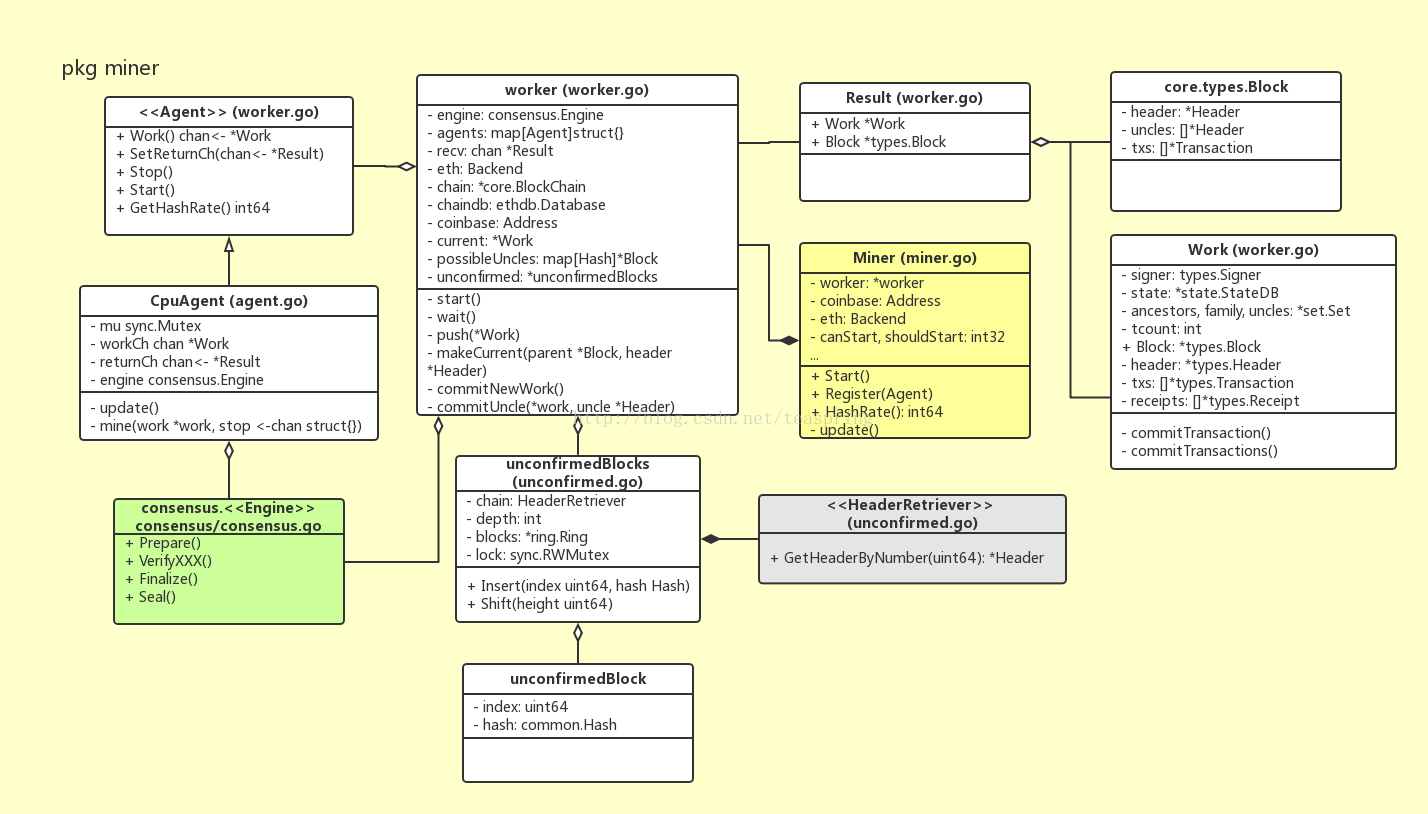
\includegraphics[scale=0.3]{miner.png}
	\caption{Miner}
	\label{miner}
\end{figure}

处于入口的类是Miner,它作为公共类型,向外暴露mine功能;它有一个worker类型的成员变量,负责管理mine过程;worker内部有一组Agent接口类型对象,每个Agent都可以完成单个区块的mine,目测这些Agent之间应该是竞争关系;Work结构体主要用以携带数据,被视为挖掘一个区块时所需的数据环境。

主要的数据传输发生在worker和它的Agent(们)之间:在合适的时候,worker把一个Work对象发送给每个Agent,然后任何一个Agent完成mine时,将一个经过授权确认的Block加上那个更新过的Work,组成一个Result对象发送回worker。

有意思的是<<Agent>>接口,尽管调用方worker内部声明了一个Agent数组,但目前只有一个实现类CpuAgent的对象会被加到该数组,可能这个Agent数组是为将来的扩展作的预留吧。CpuAgent通过全局的<<Engine>>对象,借助共识算法完成最终的区块授权。

另外,unconfirmedBlocks 也挺特别,它会以unconfirmedBlock的形式存储最近一些本地挖掘出的区块。在一段时间之后,根据区块的Number和Hash,再确定这些区块是否已经被收纳进主干链(canonical chain)里,以输出Log的方式来告知用户。

对于一个新区块被挖掘出的过程,代码实现上基本分为两个环节:一是组装出一个新区块,这个区块的数据基本完整,包括成员Header的部分属性,以及交易列表txs,和叔区块组uncles[],并且所有交易已经执行完毕,所有收据(Receipt)也已收集完毕,这部分主要由worker完成;二是填补该区块剩余的成员属性,比如Header.Difficulty等,并完成授权,这些工作是由Agent调用<Engine>接口实现体,利用共识算法来完成的。

\paragraph{新区块的组装流程}

挖掘新区块的流程入口在Miner里,略显奇葩的是,具体入口在Miner结构体的创建函数(避免称之为‘构造函数’)里。

\paragraph{共识算法完成挖掘}

共识算法族对外暴露的是Engine接口,其有两种实现体,分别是基于运算能力的Ethash算法和基于“同行”认证的的Clique算法。

\paragraph{Ethash共识算法}

Ethash算法又被称为Proof-of-Work(PoW),是基于运算能力的授权/封印过程。Ethash实现的Seal()函数,其基本原理可简单表示成以下公式:

\paragraph{Clique共识算法}
Clique算法又称Proof-of-Authortiy(PoA),它实现的Seal()其实是一个标准的数字签名加密过程,可由下列公式表示:

\ifx\allfiles\undefined
\end{document}
\fi